\documentclass[10pt,twocolumn,letterpaper]{article}

% My own stuff
\usepackage{booktabs}
% \usepackage{caption}
% \captionsetup[table]{skip=8pt}   % Only affects tables
\usepackage{stfloats}  % Add this to the preamble
\usepackage{float}

\usepackage{cvpr}
\usepackage{times}
\usepackage{epsfig}
\usepackage{graphicx}
\usepackage{amsmath}
\usepackage{amssymb}

% Include other packages here, before hyperref.

% If you comment hyperref and then uncomment it, you should delete
% egpaper.aux before re-running latex.  (Or just hit 'q' on the first latex
% run, let it finish, and you should be clear).
\usepackage[breaklinks=true,bookmarks=false]{hyperref}

\cvprfinalcopy % *** Uncomment this line for the final submission

\def\cvprPaperID{****} % *** Enter the CVPR Paper ID here
\def\httilde{\mbox{\tt\raisebox{-.5ex}{\symbol{126}}}}

% Pages are numbered in submission mode, and unnumbered in camera-ready
%\ifcvprfinal\pagestyle{empty}\fi
\setcounter{page}{1}
\begin{document}

%%%%%%%%% TITLE
\title{Primer Berbasis Data ECDO Bagian 1/2: Pemahaman Saat Ini tentang Teori Pembalikan Bumi Osilasi Dzhanibekov Pemisahan Inti-Mantel Eksotermis (ECDO)}

\author{Junho\\
Situs Web: \href{https://sovrynn.github.io}{sovrynn.github.io}\\
Repo Penelitian ECDO: \href{https://github.com/sovrynn/ecdo}{github.com/sovrynn/ecdo}\\
{\tt\small junhobtc@proton.me}
}

\maketitle
%\thispagestyle{empty}

%%%%%%%%% ABSTRACT
\begin{abstract}
Pada bulan Mei 2024, seorang penulis online dengan nama samaran “The Ethical Skeptic” \cite{0} membagikan teori revolusioner yang disebut Osilasi Dzhanibekov Pemisahan Inti-Mantel Eksotermis (ECDO) \cite{1}. Teori ini menyarankan bahwa Bumi sebelumnya telah mengalami pergeseran mendadak dan katastrofik pada poros putarnya, yang memicu banjir besar di seluruh dunia saat lautan tumpah ke benua-benua akibat kelembaman rotasi. Selain itu, ia menyajikan proses geofisika penjelasan dan data yang menunjukkan bahwa pembalikan lainnya mungkin akan terjadi. Meskipun ramalan banjir katastrofik dan kiamat semacam itu bukanlah hal baru, teori ECDO sangat menarik karena pendekatannya yang ilmiah, modern, multidisiplin, dan berbasis data.

Makalah ini adalah bagian pertama dari ringkasan dua bagian dari enam bulan penelitian independen \cite{2,20} ke dalam teori ECDO. Ini menyoroti tiga poin kunci:

\begin{flushleft}
\begin{enumerate}
    \item Pembalikan bumi mirip ECDO telah terjadi beberapa kali dalam sejarah manusia baru-baru ini, sebagaimana dibuktikan oleh mitos banjir dan tanda geologi dari banjir benua yang meluas.
    \item Arah dan besarnya perkiraan dari pembalikan Bumi di masa lalu dapat ditentukan.
    \item Data geomagnetik dan geofisika terbaru menunjukkan bahwa pembalikan Bumi lain mungkin akan terjadi, dan bahwa perubahan iklim mungkin disebabkan oleh perubahan di dalam Bumi yang lebih dalam daripada oleh manusia.
\end{enumerate}
\end{flushleft}

Selain itu, saya membahas fisika penyebab di balik pembalikan bumi yang diusulkan oleh teori ECDO.

Dalam makalah ini, saya tetap obyektif dengan berfokus pada data yang kuat, menghindari bagian teori yang menarik namun spekulatif, dan menekankan bahwa ini adalah topik yang mendesak untuk diselidiki lebih lanjut oleh umat manusia.
\end{abstract}

%%%%%%%%% BODY TEXT
\section{Pendahuluan}

Kisah tentang banjir besar bukanlah hal baru - sebenarnya, mereka ditemukan di setiap budaya besar di seluruh dunia, meliputi semua peradaban. Plotting (Gambar \ref{fig:1}) kompilasi dari 267 cerita banjir \cite{3} menunjukkan bahwa hampir semua area yang dihuni Bumi mengandung cerita tentang banjir.

\begin{figure}[h]
\begin{center}
   \includegraphics[width=1\linewidth]{b.png}
\end{center}
   \caption{Lokasi cerita banjir di seluruh dunia \cite{3}.}
\label{fig:1}
\label{fig:onecol}
\end{figure}

Pandangan lebih dekat pada cerita banjir ini menunjukkan kepada kita bahwa ini bukan banjir biasa, melainkan, bencana yang merusak diikuti dengan banjir yang membersihkan benua-benua.

\subsection{Cerita Katastrofi Penduduk Asli Amerika}

Cerita Penduduk Asli Amerika mengandung beberapa catatan paling hidup tentang bencana besar di Bumi. Suku Hopi, sebuah suku Penduduk Asli Amerika yang tinggal di timur laut Arizona, mengatakan bahwa, \textit{"..Sótuknang memanggil Orang-Orang Semut untuk membuka dunia bawah tanah mereka bagi orang-orang terpilih. Ketika mereka sudah aman di bawah tanah, Sótuknang memerintahkan si kembar, Pöqánghoya dan Palöngawhoya, untuk meninggalkan pos mereka di ujung utara dan selatan poros dunia, tempat mereka bertugas untuk menjaga agar bumi berputar dengan benar. \textbf{Si kembar hampir tidak meninggalkan pos mereka ketika dunia, tanpa ada yang mengendalikannya, terhuyung-huyung tanpa keseimbangan, berputar-putar liar, kemudian terguling dua kali.} Gunung-gunung jatuh ke laut dengan percikan besar, laut dan danau meluap melewati daratan; dan saat dunia berputar melalui ruang yang dingin dan tanpa kehidupan, ia membeku menjadi es padat"} \cite{4}.

Banyak dari cerita ini dengan tepat menggambarkan skala banjir yang masif, menceritakan bagaimana lautan naik untuk menenggelamkan semua kecuali puncak gunung tertinggi. Suku Skokomish, yang tinggal di negara bagian Washington, menceritakan bagaimana, \textit{"Roh Agung, marah dengan kebejatan manusia dan hewan, memutuskan untuk membersihkan bumi dari semua kecuali hewan baik, satu orang baik, dan keluarganya. Atas arahan Roh Agung, pria itu menembakkan anak panah ke awan, lalu anak panah lain ke anak panah itu, dan seterusnya, membuat tali panah dari awan ke tanah. Hewan dan manusia yang baik memanjat. Hewan dan ular jahat mulai memanjat, tapi pria itu memutuskan tali. \textbf{Kemudian Roh Agung menyebabkan hujan selama berhari-hari, membanjiri hingga garis salju Takhoma (Gunung Ranier).} Setelah semua manusia dan hewan jahat tenggelam, Roh Agung menghentikan hujan, air perlahan surut, dan manusia serta hewan yang baik turun"} \cite{3}. Untuk referensi, Gunung Rainier adalah gunung berapi aktif di Washington dengan puncak yang berada 4392,5 m di atas permukaan laut.

Cerita banjir dari suku Makah di negara bagian Washington secara khusus menyebutkan banjir multi-fase dari air "sangat hangat", menunjukkan bahwa ini bukan banjir biasa: \textit{"Lautan naik cukup tinggi untuk memutuskan tanjung. Kemudian ia surut, mencapai titik terendahnya empat hari kemudian, meninggalkan Teluk Neah tinggi dan kering. Kemudian ia naik kembali menutupi semua kecuali puncak gunung. \textbf{Air yang naik sangat hangat.} Orang-orang dengan kano memuat barang-barang mereka dan dibawa jauh ke utara. Banyak yang mati ketika kano mereka terjebak di pohon. Laut kembali normal setelah empat hari lagi, dan orang-orang menemukan diri mereka jauh ke utara, di mana keturunan mereka masih tinggal"} \cite{3}.

\subsection{Cerita Bencana Tiongkok}

Di sisi lain Samudra Pasifik, peradaban Tiongkok modern dikatakan dimulai dengan sebuah banjir besar. Dinasti Xia, yang diperkirakan ada sekitar tahun 2000 SM, dibentuk oleh Yu yang Agung, yang menghentikan Banjir Besar Gun-Yu \cite{6}. Pada masanya, \textit{"... dikatakan terjadi keajaiban bahwa matahari selama rentang sepuluh hari tidak terbenam, hutan-hutan terbakar, dan sejumlah besar serangga menjijikkan muncul... Gelombang besar "yang mencapai langit" jatuh di daratan Tiongkok. \textbf{"Air tersebut mencapai pegunungan tinggi, dan kaki bukit sama sekali tidak terlihat"}... "Menghancurkan dalam melimpahnya adalah air-air banjir," kata kaisar. "Dalam luasnya mereka merangkul bukit dan mengatasi ketinggian besar, mengancam langit dengan arus mereka." Kaisar memerintahkan semua usaha dilakukan untuk membuka saluran air yang tertahan di lembah di antara pegunungan. Selama bertahun-tahun penduduk bekerja keras, berusaha membebaskan dataran dan lembah dari air banjir dengan menggali saluran dan mengeringkan ladang. Selama bertahun-tahun, semua usaha sia-sia. Menteri yang bertanggung jawab atas pekerjaan yang mendesak dan besar ini, Khwan, dihukum mati karena kegagalannya... dan hanya putranya Yu yang berhasil mengeringkan tanah. Prestasi ini begitu tinggi dinilai sehingga Yu menjadi kaisar Tiongkok setelah Raja Shun, penerus pertama Yahou"} \cite{5}.

Tampaknya tidak hanya Tiongkok yang dibanjiri, tetapi ada kebutuhan untuk mengukur ulang arah mata angin dan pergerakan matahari serta bulan, yang mengisyaratkan bahwa rotasi Bumi mungkin telah berubah selama banjir: \textit{\textbf{"Kaisar ini mengirim sarjana ke berbagai bagian Tiongkok, bahkan ke Indo-Tiongkok, untuk menemukan letak utara, barat, timur, dan selatan dengan mengamati arah terbit dan terbenamnya matahari serta gerakan bintang-bintang.} Dia juga menugaskan para astronomnya untuk mencari tahu durasi musim, dan menyusun kalender baru... "Kemudian Yaou [Yahou] memerintahkan He dan Ho, dalam kepatuhan hormat terhadap langit yang luas, untuk menghitung dan menggambarkan gerakan serta penampakan matahari, bulan, bintang, dan ruang zodiak; dan untuk secara hormat menyampaikan musim kepada rakyat""} \cite{5}.

Catatan bencana dalam sejarah Tiongkok sebenarnya sudah ada jauh sebelum Dinasti Xia, bahkan mencapai era Tiga Penguasa dan Lima Kaisar \cite{7}. Nüwa, salah satu dari Tiga Penguasa dan tokoh sentral Kreasi dalam sejarah Tiongkok, menghentikan banjir selama bencana di mana Bumi berubah rotasi: \textit{"Ada pertengkaran antara dua dewa yang lebih kuat, dan mereka memutuskan untuk menyelesaikannya dengan pertarungan. Ketika dewa air Gong Gong melihat bahwa ia kalah, ia memukul kepalanya ke Gunung Buzhou, pilar yang menahan langit. \textbf{Pilar tersebut runtuh dan menyebabkan langit miring ke arah barat laut dan bumi bergeser ke arah tenggara.} Ini menyebabkan bencana besar, seperti kebakaran yang tiada henti, banjir besar, dan kemunculan binatang buas pemakan manusia. Nüwa memotong kaki kura-kura raksasa dan menggunakannya untuk menggantikan pilar yang jatuh, mengurangi situasi dan menutup langit yang pecah menggunakan batu dari tujuh warna berbeda, tetapi dia tidak dapat sepenuhnya memperbaiki langit yang miring"} \cite{8}.

\subsection{Kisah Bencana Eropa, Maya, Timur Tengah, dan Asia Tenggara}


Seperti ada terlalu banyak cerita bencana untuk dirinci dalam makalah ini, saya akan menyertakan penyebutan singkat beberapa budaya lain yang memiliki cerita seperti itu. Sastra Yunani mencakup tiga cerita banjir, yaitu Deucalion, Ogyges, dan Dardanus \cite{9,10}. Selama yang pertama, \textit{"Setelah sembilan hari banjir, dunia dihancurkan, dan bahtera beristirahat di puncak Gunung Parnassus"}, yang memiliki ketinggian puncak 2.457 meter \cite{11}. Sastra Maya meyakini ada empat Matahari yang berbeda sebelum Matahari saat ini, dan bahwa zaman Matahari keempat, Calchiuhtlicue, berakhir dengan banjir yang menghancurkan dunia sekitar 3100 SM dan kelahiran matahari kelima saat ini \cite{12}. Di Timur Tengah, kronologi Alkitab mengandung banjir Nuh yang terkenal, dan Epos Gilgamesh, sebuah puisi Babilonia, menceritakan kisah serupa \cite{13}. Budaya Asia Tenggara juga kaya dengan cerita banjir - misalnya, orang Ot Danum di Indonesia mengatakan bahwa, \textit{"Sebuah air bah besar pernah menenggelamkan banyak orang. Sedikit orang selamat dengan melarikan diri dengan perahu ke satu puncak gunung yang tersisa di atas air. Mereka tinggal di sana selama tiga bulan sampai banjir surut"} \cite{3}. Pulau Kalimantan, tempat mereka tinggal, memiliki ketinggian puncak 4.095 meter.

\begin{figure*}[t]
\begin{center}
% \fbox{\rule{0pt}{2in} \rule{.9\linewidth}{0pt}}
\includegraphics[width=1\textwidth]{marine.jpg}
\end{center}
   \caption{Peta global fosil laut (oseanik), air asin, dan tambak/tambang garam \cite{15,16,86,87}.}
   \label{fig:2}
\end{figure*}

\subsection{Analisis Statistik Cerita Bencana}

Jelas, cerita-cerita ini menggambarkan banjir besar yang sering kali disertai dengan jenis kekuatan geofisik bencana lainnya. Analisis terhadap 117 cerita bencana (Tabel \ref{tab: 1}) menunjukkan bahwa badai api, perubahan topografi, dan perubahan rotasi Bumi sering tercatat terjadi bersamaan dengan banjir besar \cite{14}:

\begin{table}[ht]
\begin{center}
\renewcommand{\arraystretch}{1.2}  % Optional, to increase row spacing
\begin{tabular}{|l|c|c|}
\hline
\textbf{Jenis Bencana} & \textbf{Jumlah} & \textbf{Kejadian} \\
\hline\hline
Air bah/banjir        & 84 & 71.79 \\
Kebakaran/badai api   & 39 & 33.33 \\
Perubahan topografi   & 29 & 24.79 \\
Gangguan bintang      & 15 & 12.82 \\
Langit runtuh         & 15 & 12.82 \\
Kegelapan berkepanjangan & 14 & 11.97 \\
Tanah dan danau hilang & 12 & 10.26 \\
Angin siklon          & 10 & 8.55  \\
Perubahan aksial/rotasi & 9 & 7.69  \\
Sungai/lautan mendidih & 8 & 6.84 \\
\hline
\end{tabular}
\end{center}
\caption{Tingkat Kejadian Efek Bencana dalam Cerita}
\label{tab: 1}
\end{table}

Spesifikasi cerita banjir yang muncul dari banyak budaya independen di seluruh dunia, bersama dengan cerita-cerita yang cocok tentang kejadian bencana lainnya, menunjukkan bahwa cerita-cerita banjir ini mungkin merupakan catatan langsung dari bencana yang benar-benar terjadi.

\section{Bukti Fisik untuk Banjir Oseanik}

Mendukung cerita banjir adalah berbagai bentuk bukti fisik dari genangan oseanik yang meluas di permukaan benua Bumi. Bentuk bukti paling langsung meliputi garam (air asin, tambak garam, dan tambang garam) dan fosil laut (oseanik), yang meliputi area besar dari daratan benua Bumi. Figure \ref
Beberapa area paling menarik yang berisi air asin adalah dataran tinggi Himalaya di Tibet dan pegunungan Andes di Amerika Selatan, kedua area tersebut memiliki ketinggian rata-rata 4000 meter, yang pertama digambarkan dalam Gambar \ref{fig:3}. Kisah banjir di Tibet menyatakan bahwa, \textit{"\textbf{Tibet hampir sepenuhnya terendam}, hingga dewa Gya merasa kasihan pada para penyintas, mengalirkan air melalui Bengal, dan mengirim guru untuk mendidik orang-orang, yang sampai saat itu tidak lebih baik dari monyet"} \cite{3}. Mitos Peru menggambarkan pembangunan gunung terjadi bersamaan dengan banjir menutupi puncak gunung: \textit{"Gembala dan enam anaknya mengumpulkan semua makanan dan domba yang mereka bisa dan membawanya ke puncak gunung yang sangat tinggi Ancasmarca. \textbf{Saat air banjir naik, gunung itu naik lebih tinggi, sehingga puncaknya tidak pernah terendam, dan gunung itu kemudian tenggelam bersama air.} Enam anak itu menghidupkan kembali provinsi itu setelah banjir"} \cite{3}.

\begin{figure}[t]
\begin{center}
   \includegraphics[width=1\linewidth]{tibet.jpg}
\end{center}
   \caption{Peta topografi Himalaya yang menunjukkan air asin (warna teal), garam kering (warna putih), dan fosil laut (warna merah) \cite{15,16,86,87}.}
\label{fig:3}
\label{fig:onecol}
\end{figure}

Sementara aliran pemikiran geologi uniformitarian mengaitkan anomali seperti garam dan fosil laut dengan proses yang terjadi dalam jutaan tahun, kisah banjir umat manusia seharusnya membuat kita mempertanyakan pemikiran tersebut. Jika laut benar-benar membanjiri benua, maka air asin dan fosil laut, yang mudah ditemukan di hamparan lahan ketinggian tinggi yang luas, adalah apa yang kita harapkan untuk ditemukan.

\begin{figure*}[t]
\begin{center}
\includegraphics[width=0.85\textwidth]{khafre.jpg}
\end{center}
   \caption{Diagram yang menunjukkan erosi karst berpola diferensial yang disebabkan oleh kenaikan tingkat laut sementara yang berlangsung lama \cite{27}.}
\label{fig:4}
\end{figure*}

\subsection{Anomali Fisik Tambahan}

Ada banyak bentuk anomali lain yang ilmu pengetahuan uniformitarian gagal menjelaskan. Mammoth yang membeku sempurna dan terjaga dengan baik terkubur dalam lumpur dengan daging yang masih dapat dimakan setelah ribuan tahun \cite{17,18,19}, lembaran besar sedimen yang disusun secara horizontal di Amerika Utara seluas 2,4 juta km$^2$ \cite{21}, lanskap ripple mega-arus \cite{22}, dan batu-batu besar yang berasal dari ratusan kilometer jauhnya terletak di puncak gunung \cite{23,26} hanyalah beberapa fenomena yang geologi uniformitarian modern abaikan dengan penjelasan umum "proses panjang dan berlangsung lama". Anomali-anomali tersebut paling baik dijelaskan melalui kekuatan geofisika yang katastrofik, dan dieksplorasi di bagian dua makalah ini.

Selain itu, ekskursi dan pembalikan kutub geomagnetik diterima secara luas sebagai fenomena berulang dari Bumi, berdasarkan data paleomagnetik \cite{35,40,41}. Namun, ilmu pengetahuan modern gagal menjelaskan secara tepat mengapa dan bagaimana pembalikan kutub ini terjadi.

\section{ECDO dan Piramida Giza}

Piramida Khafre dan Khufu di Giza adalah salah satu titik fokus utama dalam tesis ECDO oleh Ethical Skeptic \cite{27}, karena tidak hanya menyediakan bukti tentang banjir samudera yang berlangsung sementara tetapi juga menandakan potensi arah pembalikan ECDO Bumi, menunjukkan bahwa nenek moyang kita mampu mengukur bencana Bumi dan memiliki keterampilan teknik untuk menanamkan pengetahuan ini dalam struktur batu yang besar dan sangat terancang. Kedua piramida ini, diduga dibangun sekitar 2500 SM sebagai makam bagi firaun Khufu dan Khafre, keduanya terletak di Mesir utara pada kira-kira (30 N, 31 E). Mereka memiliki dasar yang panjangnya lebih dari 200 meter, dan tingginya sekitar 140 meter. Piramida Khufu dibangun menggunakan sekitar 2,3 juta blok batu kapur, masing-masing berbobot rata-rata lebih dari dua ton \cite{24, 25}.
Terdapat banyak ketidakpastian seputar asal-usul piramida-piramida ini, yang dibahas oleh Ethical Skeptic dalam tesisnya. Dia menunjukkan sejumlah ketidakkonsistenan dalam narasi konvensional seputar piramida, yang menunjukkan, paling tidak, kebingungan signifikan mengenai usia dan sejarah piramida:

\begin{flushleft}
\begin{itemize}
    \item Penanggalan karbon dari mortar kuno di sekitar dan alat pencuri makam menunjukkan bahwa piramida kemungkinan dibangun jauh lebih awal daripada yang diyakini secara konvensional.
    \item Tanda-tanda tambang yang disebut-sebut ditemukan di dalam kamar piramida Khufu terlihat mencurigakan dalam penempatan, material, keadaan preservasi, penggunaan hieroglif Mesir, dan waktu/sifat penemuan, menunjukkan bahwa mereka mungkin palsu. Mereka juga berbeda dari tanda oker kuno asli lainnya yang ditemukan di bagian lain piramida.
    \item Erosi karst diferensial pada Sphinx terdekat tidak selaras dengan narasi konvensional mengenai pembangunannya.
\end{itemize}
\end{flushleft}

\begin{figure*}[t]
\begin{center}
\includegraphics[width=0.85\textwidth]{shafts.jpg}
\end{center}
   \caption{Lorong dan kamar internal Piramida Khufu, yang diajukan oleh Ethical Skeptic sebagai observatori pemantauan geofisik tripartit untuk acara ECDO \cite{28}.}
\label{fig:5}
\end{figure*}

Salah satu area investigasi utama dalam tesis Ethical Skeptic adalah erosi berpola diferensial di bagian luar Piramida Khafre, yang digambarkan dalam Gambar \ref{fig:4}. Ujung piramida mempertahankan kerangka luar batu kapur Tura lembut aslinya, yang pernah menutupi seluruh piramida. Ujung penutup batu kapur ini sedikit pelapukan, tetapi terletak tepat di atas lapisan erosi karst berat yang sempit, mengekspos batu kapur Mokkatam Mohs 7 yang lebih keras digunakan untuk blok struktural dalam piramida. Di bawahnya, tubuh piramida mempertahankan lapisan batu kapur Tura Mohs 4 yang terkena erosi karst berat. Hal utama di sini adalah bahwa batu kapur Tura yang lebih lembut digunakan dalam casing eksternal piramida, terdiri dari CaCO$_3$, dapat larut dalam air di bawah kondisi yang tepat. Ethical Skeptic mengutip lapisan erosi karst berat selektif yang berhenti di batu kapur Mokkatam keras, erosi berpola gelombang di sudut-sudut ujung, dan perbedaan antara pelapukan ringan ujung yang terangkat dan erosi karst berat tubuh bawah piramida, sebagai bukti jelas dari peningkatan bertahap tingkat laut yang juga dengan cepat berkurang \cite{27}.

\begin{figure*}[b]
\begin{center}
\includegraphics[width=1\textwidth]{drawing.jpg}
\end{center}
   \caption{Gambaran rotasi ECDO yang diusulkan berputar 104 derajat ke utara sepanjang meridian 31 E, dengan salib menggambarkan poros timur dan barat dan penanda merah menggambarkan Piramida Khufu.}
\label{fig:6}
\end{figure*}

Ethical Skeptic juga sangat fokus pada desain internal dan kondisi piramida Khufu (Gambar \ref{fig:5}) dalam penyelidikannya \cite{28}. Piramida Khufu berisi beberapa kamar (Kamar Raja, Ratu, dan Bawah Tanah), berbagai koridor dan lorong, serta dua pasang yang disebut "lorong udara", dengan masing-masing pasangan terhubung langsung dari Kamar Raja dan Ratu \cite{29,30}. Dalam makalah ini, kami hanya akan membahas bagian paling kritis dari penyelidikan Ethical Skeptic - orientasi dan desain dari dua pasang "lorong udara", karena ini menyandikan informasi penting tentang arah pembalikan ECDO Bumi.

Hal utama di sini adalah memahami bahwa lorong-lorong itu dibangun untuk menunjuk dengan sangat tepat ke arah tertentu. Pertama-tama, kedua pasang lorong saat ini menunjuk langsung ke utara dan selatan. Selain itu, masing-masing dibangun dengan sudut dalam 104 derajat.

Petunjuk yang paling mencolok, bagaimanapun, adalah peta bintang langit yang terukir di bagian dalam salah satu poros Ratu. Peta bintang ini berpusat di sekitar orientasi kutub utara langit dari sekitar 9600 hingga 9200 SM, berdasarkan presesi ekuinoks \cite{28}. Ini menunjukkan orientasi poros yang disengaja, dan bahwa pada saat konstruksi, sepasang poros dari Kamar Raja dan Ratu menunjuk ke arah kutub utara langit. Ini menimbulkan pertanyaan - ke mana ujung-ujung lain dari poros menunjuk, dan mengapa keduanya dibangun dengan sudut 104 derajat? Etisk Skeptikus mengusulkan bahwa ini dibangun untuk sejajar dengan kutub utara langit setelah pembalikan ECDO 104 derajat.

\section{Bukti Rotasi 104 Derajat Sepanjang Meridian ke-31}

Etisk Skeptikus dengan demikian mengusulkan bahwa Bumi mengalami pembalikan 104 derajat yang berulang sepanjang meridian ke-31, di mana Piramida Khufu dan poros gandanya terletak. Gambar \ref{fig:6} menggambarkan rotasi yang diprediksi, bersama dengan "pivot" timur (Indonesia, 121 derajat T) dan barat (Amerika Selatan, 59 derajat B), dua lokasi yang tidak akan menggeser posisi setelah pembalikan sepanjang meridian ke-31. Setelah Bumi berotasi ke keadaan baru ini, diharapkan tetap di sana sebentar (beberapa dekade hingga abad) sebelum kembali ke keadaan "normal" saat ini \cite{150}.

Satu kisah kataklismik yang sangat relevan diceritakan oleh Herodotus, sejarawan paling terkenal di Yunani kuno, yang hidup pada abad kelima SM \cite{31}. Dalam bukunya "An Account of Egypt", Herodotus menceritakan bagaimana para pendeta Mesir memberitahunya, \textit{"...dari raja pertama sampai pendeta Hephaistos ini yang memerintah terakhir, telah ada tiga ratus empat puluh satu generasi manusia... tetapi tiga ratus generasi manusia setara dengan sepuluh ribu tahun, karena seratus tahun adalah tiga generasi manusia... Maka dalam periode sebelas ribu tiga ratus empat puluh tahun mereka mengatakan bahwa tidak ada dewa yang muncul dalam bentuk manusia; bahkan sebelum atau sesudahnya di antara raja-raja yang muncul di Mesir, mereka tidak melaporkan bahwa ada sesuatu semacam itu terjadi. \textbf{Pada waktu ini mereka mengatakan bahwa matahari telah bergerak empat kali dari tempatnya yang biasa terbit, dan di mana ia sekarang terbenam sejak itu dua kali telah menjadi tempat terbitnya, dan di tempat dari mana ia sekarang terbit telah dua kali menjadi tempat terbenamnya;} dan sementara itu tidak ada yang di Mesir telah berubah dari keadaan biasa, baik itu yang datang dari bumi atau yang datang kepada mereka dari sungai atau yang berkaitan dengan penyakit atau kematian"} \cite{32}. Pendeta Hephaistos dapat diberi tanggal pada awal abad ke-7 SM, seperti yang dinyatakan oleh Herodotus sendiri, sezaman dengan Sennacherib, raja dari Kekaisaran Neo-Asiria \cite{32,33,34}.

Cerita ini penting karena memberi tahu kita bahwa ketika Matahari bergerak di Mesir, ia \textit{khususnya bertukar tempat terbit dan terbenam}. Ini hanya bisa terjadi jika Mesir berbalik 180 derajat dan tetap pada garis lintang yang serupa. Ketika kami memperhitungkan desain piramida dan data yang dibahas dalam subbagian berikutnya, kita dapat menyimpulkan bahwa Mesir mungkin terletak di meridian di mana Bumi berotasi ke posisinya yang baru (meridian ke-31 timur).

Mesir adalah satu-satunya lokasi di Bumi dengan cerita yang menyebutkan bahwa Matahari secara khusus bertukar tempat terbit dan terbenam. Sebenarnya, satu-satunya cerita lain di Bumi yang merinci arah rotasi Bumi secara spesifik adalah cerita Nüwa dari Cina, yang mengatakan bahwa, \textit{"Tiang tersebut ambruk dan menyebabkan langit miring ke barat laut dan bumi bergeser ke tenggara"} \cite{8}. Arah rotasi ini juga sesuai dengan arah rotasi yang diusulkan.

\begin{figure}[b]
\begin{center}
   \includegraphics[width=0.95\linewidth]{laj.jpg}
\end{center}
   \caption{Jalur kutub geomagnetik virtual untuk (a) ekskursi Basin Iceland dan (b) ekskursi Laschamp \cite{35}.}
\label{fig:7}
\label{fig:onecol}
\end{figure}

\begin{figure*}[t]
\begin{center}
\includegraphics[width=0.9\textwidth]{biodiversity.jpg}
\end{center}
   \caption{Sebuah gambaran gurun besar di dunia dan hotspot keanekaragaman hayati yang bergantian \cite{28}.}
\label{fig:9}
\end{figure*}

\begin{figure}[t]
\begin{center}
   \includegraphics[width=1\linewidth]{meinesz3.jpg}
\end{center}
   \caption{Sebuah gambaran pola geser pada kerak Bumi \cite{36}.}
\label{fig:8}
\label{fig:onecol}
\end{figure}

\begin{figure*}[t]
\begin{center}
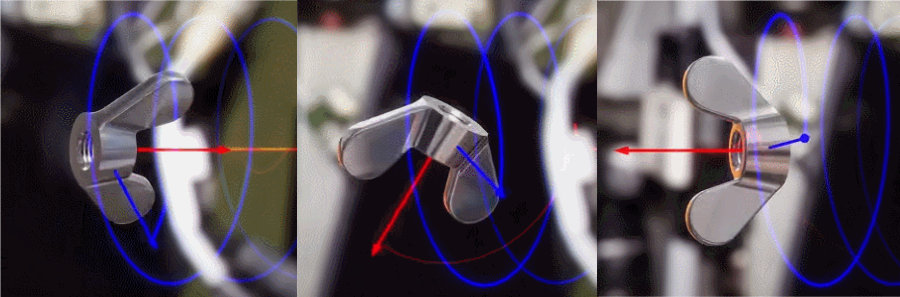
\includegraphics[width=0.9\textwidth]{dzhani.jpg}
\end{center}
   \caption{Sebuah gambaran efek Dzhanibekov \cite{28}.}
\label{fig:10}
\end{figure*}

\begin{figure*}[t]
\begin{center}
\includegraphics[width=1\textwidth]{layers.jpg}
\end{center}
   \caption{Gambaran proses inner Earth yang menyebabkan balik ECDO \cite{129}.}
\label{fig:11}
\end{figure*}

\subsection{Bukti Fisik untuk Rotasi 104 Derajat Sepanjang Meridian ke-31}

Bukti fisik yang mendukung arah rotasi ini mencakup data paleomagnetik, tektonik, gurun, keanekaragaman hayati, arus paleocurrent, dan batu pengembara glasial.

Sebuah studi data paleomagnetik yang mempertahankan jalur kutub geomagnet Basin Iceland dan ekskursi Laschamp \cite{35}, digambarkan dalam Gambar \ref{fig:7}, menunjukkan kutub-kutub berotasi kira-kira di sekitar poros ECDO timur (0 N, 121 E). Data ini direkam dalam beberapa jenis mineral magnetik di batuan yang terbentuk selama ekskursi kutub, yang mempertahankan informasi tentang arah dan intensitas medan magnet Bumi pada waktu itu.

Sebuah studi tentang bidang geser (patahan) di kerak Bumi (Gambar \ref{fig:8}), di mana kerak Bumi mengalami retakan atau deformasi, juga mengikuti pola yang sama. Felix Meinesz, seorang geofisikawan Belanda, menjelaskan dalam makalahnya \cite{36} bahwa alasan paling mungkin untuk pola ini adalah pergeseran poros rotasi Bumi.

Lokasi gurun besar dunia dan hotspot keanekaragaman hayati juga sejajar dengan pola ini. Gurun terdapat di lokasi-lokasi yang diperkirakan akan banyak dibanjiri sedimen, sementara hotspot keanekaragaman hayati berada di area yang tidak terlalu terkena perpindahan laut \cite{28}. Keselarasan ini digambarkan dalam Gambar \ref{fig:9}.

Keselarasan semacam ini terhadap jalur rotasi ECDO yang diprediksi juga ditemukan dalam paleokurensi sedimen yang diawetkan dalam lapisan batupasir di barat Amerika Serikat \cite{21}, dan batuan es yang tertinggal, yang merupakan batuan yang telah diambil, diharapkan oleh gletser, dan disimpan di tempat lain di atas batuan dasar yang berbeda dari jenis batuan awal. Di Britania Raya, batuan ini mengikuti jalur aliran yang diharapkan sesuai dengan rotasi ECDO \cite{67,68}.

\section{Fisika Penyebab Di Balik Pembalikan ECDO}

Prinsip di balik perubahan cepat poros rotasi Bumi terletak pada fisika benda berputar. Contoh kanonik dari hal ini adalah efek Dzhanibekov, ditemukan oleh astronaut Rusia Vladimir Dzhanibekov \cite{37}, dan digambarkan dalam Gambar \ref{fig:10}. Sebuah objek yang tidak berputar sempurna pada salah satu dari tiga sumbu inersianya yang utama tidak akan mempertahankan sumbu rotasi tetap. Jika ia berputar dekat dengan sumbu utama keduanya, maka objek tersebut akan mengalami apa yang tampaknya sebagai pergeseran rotasi mendadak. Meskipun ini tidak persis seperti yang kami percaya terjadi selama pembalikan cepat Bumi, intinya adalah bahwa tanpa adanya gaya eksternal, hanya fisika rotasi yang dapat menjelaskan perubahan cepat dalam sumbu rotasi Bumi.

\begin{figure}[t]
\begin{center}
   \includegraphics[width=1\linewidth]{llvp.jpg}
\end{center}
   \caption{Visual detail LLVP di bawah Afrika Selatan \cite{28}.}
\label{fig:12}
\label{fig:onecol}
\end{figure}

Secara spesifik, Bumi hampir pasti tidak mengalami efek Dzhanibekov yang sederhana dan seragam. Jika hal ini terjadi, kita akan dapat mendeteksi pergeseran bertahap dalam sumbu rotasi Bumi seiring waktu. Sebaliknya, kami percaya bahwa Bumi mengalami gangguan mendadak berkala dalam struktur fisiknya, yang menyebabkan pemisahan dari "rotasi luar" (kerak/mantel) dan "badan rotasi dalam" (inti). Tanpa masukan eksternal, hukum kekekalan momentum sudut menyatakan bahwa Bumi tidak dapat tiba-tiba mengubah sumbu rotasinya, jadi pemisahan antara badan rotasi luar dan dalam adalah salah satu dari beberapa hal, kecuali sebuah dampak eksternal pada Bumi, yang dapat menyebabkan pembalikan tiba-tiba dan mendadak.
Yang mendorong gangguan internal di Bumi diyakini adalah perubahan keadaan dalam struktur besi yang membentuk inti Bumi (Gambar \ref{fig:11}). Inti dalam terdiri dari Besi (Fe) rapat heksagonal \cite{141}. Ketika hcp-Fe ini diubah menjadi keadaan metalik cair, ia melepaskan energi kinetik, dan terpantul ke dalam inti luar. Perubahan fase ini mengurangi permeabilitas magnetik inti, melemahkan medan geomagnetik, dan melepaskan panas, menciptakan struktur LLVP (provinsi geser kecepatan rendah besar) (Gambar \ref{fig:12}) \cite{38} di mantel, dan menghangatkan permukaan Bumi melalui lautan abyssal. Kedua tren telah terdokumentasi dengan baik dalam beberapa abad terakhir dan dibahas lebih lanjut dalam makalah ini.

Proses yang sama di dalam Bumi, yang terjadi secara terbalik, juga diyakini mendorong peralihan kembali ke keadaan rotasi Bumi saat ini relatif segera setelah flip terjadi.

\section{Bukti untuk Pembalikan Bumi yang Akan Datang}

Ada alasan kuat untuk meyakini bahwa kita berada di ambang pembalikan Bumi lainnya. Sebuah bencana belum terjadi selama beberapa milenium, yang kira-kira adalah frekuensi di mana peristiwa ini tampaknya terjadi berdasarkan catatan sejarah dan data. Data terkuat yang mendukung pembalikan yang akan datang berasal dari data geomagnetik terbaru, yang menunjukkan bahwa medan geomagnetik Bumi telah melemah selama sekitar dua ribu tahun. Pelemahan ini semakin cepat dan telah mencapai tingkat yang mengkhawatirkan dalam beberapa dekade terakhir.

Digambarkan dalam Gambar \ref{fig:14} adalah medan geomagnetik Bumi pada tahun 1590 dan 2025 \cite{125,126}. Seperti yang ditunjukkan dalam gambar, medan tersebut telah melemah secara signifikan.

Metrik lain untuk melemahnya medan geomagnetik adalah posisi kutub utara geomagnetik (Gambar \ref{fig:13}). Kutub utara geomagnetik secara historis berlokasi di Arktika Kanada. Namun, telah berkelana perlahan selama beberapa abad terakhir, dan meningkat secara signifikan beberapa dekade yang lalu. Sekarang bergerak cepat menuju Rusia dengan kecepatan 55 kilometer per tahun \cite{124}.

\begin{figure}[t]
\begin{center}
   \includegraphics[width=1\linewidth]{npw.jpg}
\end{center}
   \caption{Posisi kutub utara geomagnetik dari tahun 1590 hingga 2025, digambarkan dalam kenaikan 5 tahun \cite{142}.}
\label{fig:13}
\label{fig:onecol}
\end{figure}

\begin{figure*}[t]
\begin{center}
\includegraphics[width=0.9\textwidth]{saa.jpg}
\end{center}
   \caption{Gambaran pelemahan medan geomagnetik dari tahun 1590 hingga 2025. Dihitung menggunakan model gufm1 dan IGRF-14 \cite{125,126}.}
\label{fig:14}
\end{figure*}

\begin{figure}[t]
\begin{center}
   \includegraphics[width=1\linewidth]{ocean-highlight.jpg}
\end{center}
   \caption{Tingkat pemanasan laut dalam ($>$2000 m kedalaman) dari tahun 1991 hingga 2010, dilingkari merah \cite{132}.}
\label{fig:15}
\label{fig:onecol}
\end{figure}

Medan magnetik Bumi diyakini dihasilkan oleh dinamo dalam - kolom sirkular arus magma yang bergerak di inti luar Bumi karena rotasinya \cite{123}. Medan geomagnetik yang melemah adalah gejala dari gangguan dalam di dalam Bumi. Menurut teori ECDO, gangguan ini mengeluarkan panas dan akhirnya menyebabkan pemisahan antara mantel dan inti, menyebabkan pembalikan Bumi \cite{1}.
Ada data yang cukup banyak yang menguatkan keberadaan proses eksotermis di dalam Bumi. Pemanasan Bumi terdokumentasi dalam peningkatan suhu permukaan benua dan lautan \cite{127,128}, peningkatan level CO2 atmosfer yang bergerak seiring dengan semburan panas Bumi \cite{129,130}, dan penurunan luas es laut global \cite{131}. Data menunjukkan bahwa peningkatan kadar CO2 dan suhu bukanlah penyebab perubahan iklim "buatan manusia" melainkan, dampak hilir dari inti eksotermis \cite{129}.

Yang paling signifikan, studi tentang laju pemanasan di laut dalam (kedalaman $>$2000 meter) menunjukkan bahwa tidak hanya samudera dalam yang memanas, laju pemanasan terkuat ditemukan di lapisan abyssal (4000 - 6000 m). Pemanasan laut dalam ini memiliki centroid di bawah 4000 meter \cite{132,129}, yang tidak akan mungkin terjadi jika lautan dipanaskan dari atas oleh atmosfer. Data semacam ini memberikan dukungan kuat pada kasus bahwa perubahan iklim dan geomagnetik terbaru didorong oleh proses yang terjadi jauh di dalam Bumi. Gambar \ref{fig:15} menggambarkan laju pemanasan laut dalam global dari tahun 1991 hingga 2010 \cite{132}.

\section{Pemodelan Pembalikan Bumi yang Akan Datang}

\begin{figure}[t]
\begin{center}
   \includegraphics[width=1\linewidth]{saa-crop.jpeg}
\end{center}
   \caption{Perhitungan titik balik berdasarkan Anomali Atlantik Selatan menunjukkan tanggal 13 Maret 2059 \cite{125,126}.}
\label{fig:16}
\label{fig:onecol}
\end{figure}

Memperkirakan waktu pembalikan Bumi berikutnya adalah tugas yang kompleks. Saat ini, model terbaik yang kita miliki untuk ini terletak pada medan geomagnetik Bumi - Anomali Atlantik Selatan (SAA). Wilayah ini di atas Atlantik Selatan memiliki kekuatan medan geomagnetik paling lemah dan didefinisikan sebagai area dengan kekuatan medan di bawah 32.000 nanotesla \cite{135}, yang merupakan nilai medan terlemah pada tahun 1590. Luas permukaan Anomali Atlantik Selatan meningkat dari 1\% dari permukaan Bumi pada tahun 1590 menjadi 21\% pada tahun 2025 \cite{136}.

Untuk mendapatkan perkiraan kapan Bumi bisa berbalik, saya menyesuaikan data luas permukaan SAA dengan persamaan titik balik hukum pangkat, yang memodelkan sistem kompleks yang mendekati transisi kritis, di mana sistem mengalami perubahan dramatis dan mendadak. Perhitungan saya menghasilkan tanggal titik balik yang diprediksi 13 Maret 2059 (Gambar \ref{fig:16}). Prediksi ini akan menjadi semakin akurat semakin dekat kita dengan transisi tersebut \cite{136}.

Metrik lain seperti pergerakan sumbu rotasi, anomali cuaca, dan data seismik serta vulkanik juga dapat membantu kita mendapatkan prediksi yang lebih baik tentang kapan pembalikan Bumi berikutnya mungkin terjadi.

\section{Linimasa Historis ECDO}

Meski sulit untuk menetapkan linimasa yang tepat untuk peristiwa ECDO masa lalu, tampaknya ada setidaknya 2 peristiwa ECDO selama Holosen. Perhatikan catatan yang diceritakan oleh Herodotus dari imam-imam Mesir bahwa, \textit{"dari raja pertama hingga imam Hephaistos yang berkuasa terakhir, ada tiga ratus empat puluh satu generasi manusia... Dalam waktu ini mereka mengatakan bahwa matahari telah bergerak empat kali dari tempat kebiasaannya terbit, dan di mana ia sekarang terbenam ia pernah dua kali terbit, dan di tempat dari mana ia sekarang terbit ia dua kali terbenam"} \cite{32}. Plato, yang hidup selama abad kelima SM \cite{111}, menyatakan bahwa setelah banjir yang menenggelamkan Atlantis dalam satu hari dan malam 9.000 tahun sebelumnya, \textit{"sejak saat itu telah ada banyak banjir, dan mereka yang selamat di pegunungan tidak mengetahui seni menulis, dan selama banyak generasi sepenuhnya didedikasikan untuk mendapatkan sarana hidup"} \cite{112}, yang menunjukkan ada lebih dari dua kali pembalikan sejak akhir Zaman Muda Dryas sekitar 9700 SM. Bukti fisik yang dibahas sepanjang makalah ini dan dalam penelitian saya \cite{2} memberikan banyak bukti untuk catatan Plato.

Tanggal kandidat terbaru untuk flip ECDO adalah selama periode 2300 hingga 1600 SM, di mana banyak catatan banjir kataklismik (Gun-Yu \cite{113,114,115}, Ogyges \cite{116,117}, Peru \cite{118,119}, Exodus \cite{120}), penghancuran dan pengabaian peradaban (Mohenjo-Daro \cite{121}, Minoan Kreta\cite{100,101}) dan anomali fisik (peristiwa bond \cite{122}, peristiwa 4.2 kilotahun \cite{90}) telah diberi tanggal. Tidak ada cukup banyak konvergensi bukti yang lebih baru dari ini yang menunjukkan peristiwa katastropik besar.

\section{Kesimpulan}

Operasi NANOOK adalah usaha pengintaian Perang Dingin Amerika Serikat untuk memetakan Arktik dan Pesisir Utara Soviet setelah Perang Dunia II \cite{137}. Selama penyelidikan mereka, mereka menemukan bahwa kutub magnetik berjarak 125 hingga 200 mil utara dari tempat seharusnya berdasarkan temuan dari ekspedisi sebelumnya. Karenanya, \textit{"Di antara ilmuwan pemerintah, muncul pertanyaan tentang apa yang akan terjadi ketika kutub magnetik dan geografis bertepatan. Untuk menjawab ini, di bawah kendali proyek Dr. Paul A. Siple, Rand Corporation dikontrak untuk melakukan studi di laboratorium menggunakan model bumi yang dibangun dari bola konsentris - satu bola bagian dalam mewakili inti besi cair yang bermuatan elektromagnetik dari bumi yang sumbunya mendefinisikan kutub “magnetik”; dan bola luar mewakili kerak bumi yang berputar di sekitar sumbu kutub “geografis”. Ditetapkan melalui percobaan berulang bahwa ketika kutub “magnetik” mendekati kutub “geografis”, kutub “magnetik” pada titik tertentu akan mempercepat laju konvergensinya seolah-olah ditarik ke arah kutub “geografis” oleh gaya sentripetal dan meloncat untuk bertepatan; tetapi bukannya kutub-kutub tersebut bertepatan, kutub “magnetik” akan dengan cepat “membalik” di sekitar kutub “geografis”, lalu berputar menuju ekuator seolah-olah oleh gaya sentrifugal, berakhir pada posisi di mana kedua sumbu mengasumsikan divergensi sekitar 89 derajat. Setelah “flip” kutub ini terjadi, sumbu kemudian akan secara bertahap mulai berkumpul kembali dalam jangka waktu yang panjang"} \cite{138,139}.

Selanjutnya, \textit{"Pada salah satu pertemuan ilmiah yang dihadiri Mayor White di Pentagon pada awal 1948, para ilmuwan membahas kebijakan memperingatkan publik tentang fenomena flip kutub yang akan datang. Tidak ada ilmuwan yang setuju untuk menahan informasi dari publik; tetapi, di sisi lain, mereka juga tidak dapat sepakat tentang bagaimana merilisnya. Pengetahuan tentang fenomena ini, menurut beberapa orang, dapat dengan sendirinya menghancurkan serat moral masyarakat. Ketakutan mereka ternyata tidak berdasar ketika, pada awal 1950-an, informasi tentang fenomena flip dirilis dalam kolom surat kabar dan artikel majalah, tetapi mengejutkan tidak menghasilkan tanggapan dari publik yang tampaknya terkejut, parokial atau tidak percaya"} \cite{138,139}.

Mengapa kita tidak memperhatikan ini? Ada banyak alasan untuk percaya bahwa Bumi pernah terbalik sebelumnya. Makalah ini, bersama dengan bagian kedua dari makalah, memberikan ringkasan padat dari konvergensi bukti besar dari berbagai bidang yang menunjukkan bahwa ini adalah kasusnya, seperti cerita banjir di seluruh dunia, fosil garam dan laut yang menutupi benua, tempat perlindungan bawah tanah kuno, sisa-sisa hewan, dan lanskap geologis kataklismik. Manusia seharusnya berusia ratusan ribu tahun, namun sejarah modern hanya berlangsung beberapa ribu tahun. Mungkinkah setiap kali, Bumi berbalik, benua-benua dibersihkan, dan kita dipaksa kembali ke titik awal - Zaman Batu - mengurangi catatan sejarah kuno kita menjadi segelintir cerita kataklismik? Jika demikian, maka mencegah hal ini terjadi lagi mungkin merupakan salah satu tugas terpenting umat manusia.
Sebagai penutup, saya akan meninggalkan Anda dengan kisah yang diceritakan dalam Timaeus, yang ditulis oleh Plato, tentang percakapan antara Solon, seorang negarawan Athena, dan para pendeta Mesir \cite{140}: \textit{"Dan pada suatu kesempatan, ketika [Solon] ingin menarik mereka untuk berdiskusi tentang sejarah kuno, dia mencoba menceritakan kepada mereka tradisi paling kuno kami, tentang Phoroneus, yang dikatakan sebagai manusia pertama, dan Niobe; dan dia melanjutkan untuk menceritakan legenda tentang Deucalion dan Pyrrha setelah Banjir, dan bagaimana mereka selamat dari itu, dan memberikan silsilah keturunan mereka; dan dengan menceritakan jumlah tahun yang ditempuh oleh peristiwa-peristiwa yang disebutkan, dia mencoba menghitung periode waktu. Ketika salah satu pendeta, orang yang sangat tua sekali, berkata, “Wahai Solon, Solon, kalian orang Yunani selalu anak-anak: tidak ada orang Yunani yang tua.” Dan setelah mendengar ini dia bertanya, “Apa yang Anda maksud dengan perkataan ini?” Dan pendeta itu menjawab, “Kalian muda dalam jiwa, masing-masing dari kalian. Karena di dalamnya kalian tidak memiliki satu keyakinan pun yang kuno dan berasal dari tradisi lama, maupun satu ilmu pun yang beruban dengan usia. Dan ini adalah penyebabnya: Telah ada dan akan ada banyak dan berbagai kehancuran umat manusia, yang terbesar adalah oleh api dan air, dan yang lebih kecil oleh banyak cara lainnya yang tak terhitung banyaknya. Karena sebenarnya cerita yang diceritakan di negaramu maupun di negara kami, bagaimana dahulu kala Phaethon, putra Helios, mengaitkan kereta ayahnya, dan, karena dia tidak mampu mengemudikannya sepanjang jalan yang diambil oleh ayahnya, membakar semua yang ada di bumi dan dia sendiri binasa oleh petir — cerita itu, sebagaimana diceritakan, memiliki corak legenda, tetapi kebenarannya terletak pada terjadinya pergeseran tubuh di langit yang bergerak mengelilingi bumi, dan kehancuran benda-benda di bumi oleh api yang ganas, yang terjadi pada interval panjang. Pada saat-saat ini semua yang tinggal di pegunungan dan di tempat tinggi dan kering menderita kehancuran lebih daripada mereka yang tinggal dekat sungai atau laut; dan dalam kasus kami, Sungai Nil, Penyelamat kami dalam berbagai cara, menyelamatkan kami juga pada saat-saat ini dari bencana ini dengan naik tinggi. Dan ketika, di sisi lain, para Dewa membersihkan bumi dengan banjir air, semua gembala dan penggembala yang berada di pegunungan diselamatkan, tetapi mereka yang berada di kota-kota di negaramu tersapu ke laut oleh arus; sedangkan di negara kami tidak pernah terjadi ataupun pada waktu lain air mengalir deras menutupi ladang dari atas, sebaliknya semua cenderung alami untuk muncul dari bawah. Oleh karena itu, untuk alasan-alasan ini, yang dilestarikan di sini dianggap paling kuno; kebenarannya adalah bahwa di setiap tempat di mana tidak ada panas atau dingin yang berlebihan untuk mencegahnya selalu ada beberapa keturunan manusia, sekarang lebih banyak, sekarang lebih sedikit jumlahnya. Dan jika ada peristiwa yang terjadi yang mulia atau besar atau dalam cara apa pun mencolok, apakah itu di negaramu atau di negara kami atau di tempat lain yang kami ketahui dari laporan, semua peristiwa semacam itu dicatat dari zaman dahulu dan disimpan di sini di dalam kuil kami; sedangkan orang-orangmu dan yang lainnya baru dilengkapi, setiap kali, dengan huruf dan semua seni semacam itu yang diperlukan oleh Negara-negara beradab dan ketika, setelah jeda tahun biasa, seperti wabah, banjir dari langit datang melanda ke bawah pada orang-orangmu, tidak meninggalkan satupun dari kalian kecuali yang buta huruf dan tidak berbudaya, sehingga kalian menjadi muda seperti sebelumnya, tanpa pengetahuan tentang semua yang terjadi di masa lampau di negeri ini atau di negeri kalian sendiri. Tentu saja silsilah-silsilah yang baru saja kau ceritakan tadi, Solon, tentang orang-orang dari negaramu, sedikit lebih baik daripada dongeng anak-anak; karena, pertama-tama, kamu hanya mengingat satu banjir, padahal banyak yang telah terjadi sebelumnya; dan selanjutnya, kamu tidak menyadari kenyataan bahwa ras paling mulia dan sempurna di antara manusia lahir di tanah di mana kamu sekarang tinggal, dan dari mereka baik kamu sendiri maupun seluruh kotamu yang sekarang ada, berasal dari beberapa benih kecil yang kebetulan tersisa; tetapi ini telah luput dari pengamatanmu karena selama banyak generasi orang-orang yang selamat meninggal tanpa kemampuan untuk mengungkapkan diri mereka dalam tulisan. Karena sesungguhnya pada suatu waktu, Solon, sebelum kehancuran terbesar oleh air, apa yang sekarang menjadi Negara Athena adalah yang paling berani dalam perang dan juga sangat terorganisir dalam segala hal lainnya. Dikatakan bahwa ia memiliki karya seni yang paling megah dan kebijakan paling mulia dari bangsa mana pun di bawah langit yang telah kami dengar.”}.
Para pendeta yang sama ini, tentu saja, juga memberi tahu Solon tentang peradaban kuno Atlantis: \textit{"Karena semua yang kita miliki di sini, terletak di dalam mulut yang kita bicarakan, jelas merupakan pelabuhan yang memiliki pintu masuk sempit; tetapi di luar sana adalah lautan sejati, dan tanah yang mengelilinginya dengan tepat dapat disebut, dalam arti yang paling penuh dan paling benar, sebuah benua. Sekarang di pulau Atlantis ini ada sebuah konfederasi raja, dengan kekuasaan besar dan menakjubkan, yang menguasai seluruh pulau, dan juga banyak pulau lainnya dan bagian dari benua; dan, lebih-lebih lagi, dari tanah di sini dalam Selat mereka menguasai Libya sampai ke Mesir, dan atas Eropa sampai ke Tyrrhenia. Jadi tuan rumah ini, yang semuanya berkumpul, mencoba sekali waktu untuk memperbudak dengan satu serangan baik negara Anda maupun negara kami dan seluruh wilayah di dalam Selat. Dan kemudian, Solon, saat itulah keberanian negara Anda menunjukkan dirinya menonjol dalam keberanian dan kekuatan di hadapan seluruh dunia. Karena berdiri terkemuka di atas semua dalam keberanian dan semua seni perang, dan sebagian bertindak sebagai pemimpin orang-orang Yunani, dan sebagian berdiri sendiri ketika ditinggalkan oleh semua yang lain, setelah menghadapi bahaya mematikan, mengalahkan para penyerbu dan membangun sebuah trofi; dengan cara itu menyelamatkan dari perbudakan mereka yang belum diperbudak, dan semua yang lain dari kita yang tinggal di dalam batas-batas Heracles dibebaskan tanpa pamrih. Tetapi pada waktu kemudian terjadi gempa bumi dan banjir besar yang mengerikan, dan satu hari dan malam yang menyedihkan menimpa mereka, ketika seluruh tubuh para pejuang Anda ditelan oleh bumi, dan pulau Atlantis dengan cara serupa ditelan oleh laut dan lenyap"}.

\section{Ucapan Terima Kasih}

Terima kasih kepada Ethical Skeptic, penulis asli tesis ECDO, atas penyelesaian tesisnya yang penuh wawasan dan inovatif serta membagikannya dengan dunia. Tesisnya yang terdiri dari tiga bagian \cite{1} tetap menjadi karya seminal untuk teori Exothermic Core-Mantle Decoupling Dzhanibekov Oscillation (ECDO), dan mengandung lebih banyak informasi tentang topik ini daripada yang saya bahas secara singkat di sini.

Terima kasih kepada Ankit, yang memproses data kompilasi bencana di Tabel 1.

Dan tentu saja, terima kasih kepada para raksasa yang di pundaknya kita berdiri; mereka yang telah melakukan semua penelitian dan penyelidikan yang membuat karya ini mungkin dan berusaha membawa cahaya bagi kemanusiaan.

\clearpage
\twocolumn

\section{Gambar Tambahan}

\begin{figure}[H]
\begin{center}
   \includegraphics[width=1\linewidth]{wave.jpg}
\end{center}
   \caption{Pandangan dekat terhadap erosi gelombang parabola di piramida Khafre \cite{27}.}
\label{fig:19}
\label{fig:onecol}
\end{figure}

\begin{figure}[H]
\begin{center}
   \includegraphics[width=1\linewidth]{star-stone.jpg}
\end{center}
   \caption{Peta bintang yang terukir di batu di salah satu terowongan piramida Khufu \cite{28}.}
\label{fig:20}
\label{fig:onecol}
\end{figure}

\begin{figure*}[t]
\begin{center}
\includegraphics[width=1\textwidth]{deepsea.jpg}
\end{center}
   \caption{Visual anomali pemanasan lautan dalam dan abyssal dibandingkan dengan kurva pemanasan lautan atmosfer normal. Anomali pemanasan keseluruhan diambil dari NOAA \cite{147}, distribusi pemanasan dalam dan abyssal dari studi Desbruyeres \cite{132}, dan pemrosesan data serta visualisasi oleh Ethical Skeptic \cite{129}.}
\label{fig:21}
\end{figure*}

\begin{figure*}[t]
\begin{center}
\includegraphics[width=1\textwidth]{sealevel.jpeg}
\end{center}
   \caption{Tingkat permukaan laut menunjukkan peningkatan varians 20\% selama 75 tahun di 63 stasiun, menunjukkan peningkatan kecepatan arus. Angkatan varians permukaan laut bersamaan dengan nadi panas lautan, menunjukkan bahwa keduanya mungkin disebabkan oleh pemanasan dari bawah laut Bumi \cite{2,129}.}
\label{fig:22}
\end{figure*}

\begin{figure*}[t]
\begin{center}
\includegraphics[width=1\textwidth]{co2.jpg}
\end{center}
   \caption{Ppm CO2 atmosfer telah meningkat secara konsisten selama 45 tahun terakhir, kemungkinan disebabkan oleh kenaikan suhu laut. Sumber: NOAA \cite{148,129}.}
\label{fig:23}
\end{figure*}

\begin{figure*}[t]
\begin{center}
\includegraphics[width=1\textwidth]{ice.jpg}
\end{center}
   \caption{Luas es laut global telah menyusut selama 45 tahun terakhir, akibat pemanasan bumi. Sumber: ADS \cite{149}.}
\label{fig:24}
\end{figure*}

\clearpage
\twocolumn

{\small
\bibliographystyle{ieee}
\bibliography{egbib}
}

\end{document}
